%%%%%%%%%%%%%%%%%%%%%%%%%%%%%%%%%%%%%%%%%%%%%%%%%%%%%%%%%%%%%%%%%%%%%%%%%%%%%%%
% Rownanie na faze
%%%%%%%%%%%%%%%%%%%%%%%%%%%%%%%%%%%%%%%%%%%%%%%%%%%%%%%%%%%%%%%%%%%%%%%%%%%%%%%
\newpage
\subsection{Ruch jednostajnie przyspieszony.}
W przypadku relatywistycznego odpowiednika ruchu jednostajnie 
przyspieszonego mamy $\chi = \pi$ oraz $\alpha = const$.
W tym przypadku analityczne rozwiązanie 
równania na fazę zegara jest postaci
\begin{align*}
\varphi = \pi + 
2\text{arctg} \left( 
\sqrt{1-\frac{\alpha^2\ell^2}{4}} 
\text{tg} \left( \pm 
\sqrt{1-\frac{\alpha^2\ell^2}{4}} 
(s + s_0)/\ell\right)  \mp \frac{\alpha \ell}{2}
\right),
\end{align*}
gdzie
\begin{align*}
s_0 & = \pm \ell \text{arctg}  
\left( \left(1 \pm\frac{\alpha\ell}{2}\right) \Big / 
\sqrt{1-\frac{\alpha^2\ell^2}{4}}  \right)
\Big /\sqrt{1-\frac{\alpha^2\ell^2}{4}} ,
\end{align*}
natomiast przybliżone rozwiązanie 
\begin{align*}
\varphi =  \pm \frac{2}{\ell}s - \frac{\pi}{2} 
+ \frac{\alpha \ell}{2}  \sin (2 s / \ell  )  
+O(\alpha^2).
\end{align*}
Rozwiązania dla $\ell=0,01$ oraz $\alpha=100$ przy różnych 
kierunkach działania zegara 
zostały przedstawione na wykresach~\ref{fig:1a}-\ref{fig:1d}.
Wykres pełnego rozwiązania ukazuje, 
że niezależnie od kierunku działania zegara przy dużych 
przyspieszeniach zegar będzie opóźniony w stosunku do
czasu własnego. Tego efektu nie widać w rozwiązaniu przybliżonym.
Na wykresach~\ref{fig:2a1}-\ref{fig:2n3} porównano przybliżone rozwiązanie
 z~pełnym dla różnych przyspieszeń. 
Widzimy, że przybliżenie jest zadowalające dla odpowiednio małych 
wartości $\epsilon = \alpha / \alpha_c$.
\begin{figure}[h]
\begin{minipage}[b]{.5\linewidth}
\centering
\includegraphics[scale=0.52]{HiperAppA100L2.eps}
\subcaption{Przybliżone rozwiązanie}\label{fig:1a}
\end{minipage}%
\begin{minipage}[b]{.5\linewidth}
\centering
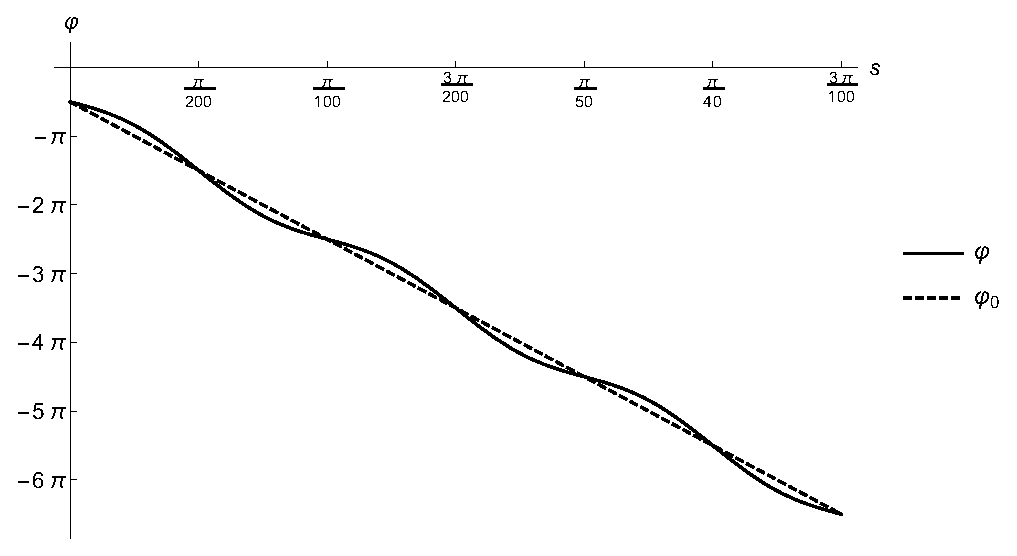
\includegraphics[scale=0.52]{HiperAppA100L2M.eps}
\subcaption{Przybliżone rozwiązanie w odwrotnym działaniu zegara}\label{fig:1b}
\end{minipage}
\begin{minipage}[b]{.5\linewidth}
\centering
\includegraphics[scale=0.52]{HiperNumA100L2.eps}
\subcaption{Pełne rozwiązanie}\label{fig:1c}
\end{minipage}%
\begin{minipage}[b]{.5\linewidth}
\centering
\includegraphics[scale=0.52]{HiperNumA100L2M.eps}
\subcaption{Pełne rozwiązanie w odwrotnym działaniu zegara}\label{fig:1d}
\end{minipage}
\caption{Faza zegara $\varphi$ w ruchu hiperbolicznym dla 
$\ell=0,01$ oraz $\alpha=100$ w porównaniu do fazy 
$\varphi_0$ w układzie bez przyspieszeń. }\label{fig:1}
\end{figure}
\begin{figure}
\begin{minipage}[b]{.5\linewidth}
\centering
\includegraphics[scale=0.52]{HiperAppA25L2.eps}
\subcaption{Przybliżone rozwiązanie dla $\alpha=25$}\label{fig:2a1}
\end{minipage}%
\begin{minipage}[b]{.5\linewidth}
\centering
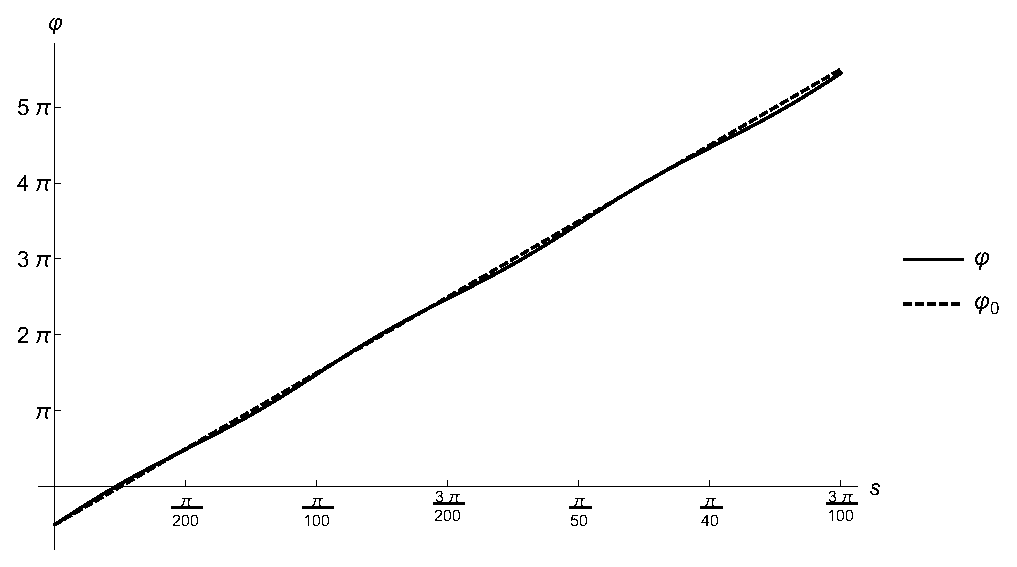
\includegraphics[scale=0.52]{HiperNumA25L2.eps}
\subcaption{Pełne rozwiązanie dla $\alpha=25$}\label{fig:2n1}
\end{minipage}
\begin{minipage}[b]{.5\linewidth}
\centering
\includegraphics[scale=0.52]{HiperAppA50L2.eps}
\subcaption{Przybliżone rozwiązanie dla $\alpha=50$}\label{fig:2a2}
\end{minipage}%
\begin{minipage}[b]{.5\linewidth}
\centering
\includegraphics[scale=0.52]{HiperNumA50L2.eps}
\subcaption{Pełne rozwiązanie dla $\alpha=50$}\label{fig:2n2}
\end{minipage}
\begin{minipage}[b]{.5\linewidth}
\centering
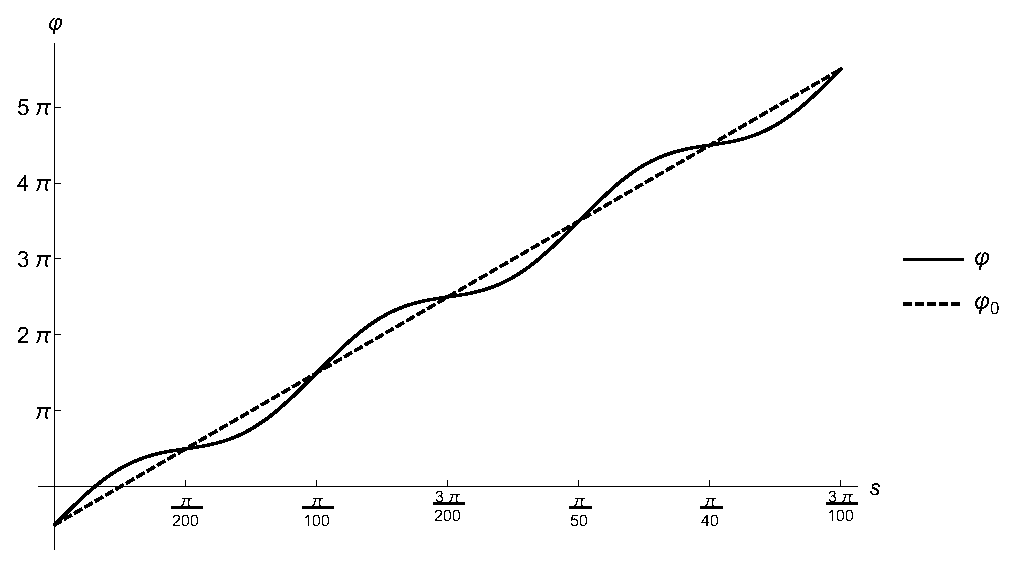
\includegraphics[scale=0.52]{HiperAppA150L2.eps}
\subcaption{Przybliżone rozwiązanie dla $\alpha=150$}\label{fig:2a3}
\end{minipage}%
\begin{minipage}[b]{.5\linewidth}
\centering
\includegraphics[scale=0.52]{HiperNumA150L2.eps}
\subcaption{Pełne rozwiązanie dla $\alpha=150$}\label{fig:2n3}
\end{minipage}
\caption{Porównanie rozwiązania przybliżonego z rozwiązaniem pełnym
dla fazy zegara $\varphi$ w ruchu hiperbolicznym przy
$\ell=0,01$. Linią przerywaną zaznaczono fazę 
$\varphi_0$ w układzie bez przyspieszeń. }\label{fig:2}
\end{figure}


\subsection{Ruch po okręgu.}
W przypadku ruchu po okręgu o promieniu $R$ z 
częstością $\omega$ mamy
$\chi = \omega \gamma^2 s$ oraz 
$\alpha = R\omega^2\gamma^2 $.
W takim przypadku rozwiązanie równania na fazę zegara dane jest przez
\begin{align}\nonumber
\varphi = \omega\gamma^2 s +  
2\text{arctg} \left( 
\sqrt{ 1-\frac{R^2\omega^4\gamma^4}{\left( \pm \frac{2}{\ell} 
-\omega\gamma^2 \right)^2 } }
\text{tg} \left( 
\left( \pm \frac{2}{\ell} -\omega\gamma^2 \right)
\sqrt{ 1-\frac{R^2\omega^4\gamma^4}{\left( \pm \frac{2}{\ell} 
-\omega\gamma^2 \right)^2 } }(s + s_0)/2
\right)  
- \frac{R \omega^2 \gamma^2}{\pm \frac{2}{\ell} -\omega\gamma^2}
\right),
\end{align}
gdzie
\begin{align*}
s_0 & = \frac{2}{\pm \frac{2}{\ell} -\omega\gamma^2} 
\text{arctg}  
\left( \left( \frac{R \omega^2 \gamma^2}{\pm \frac{2}{\ell} 
-\omega\gamma^2} - 1 \right) \Big /  
\sqrt{ 1-\frac{R^2\omega^4\gamma^4}{\left( \pm \frac{2}{\ell} 
-\omega\gamma^2 \right)^2 } }
\right)\Big /   
\sqrt{ 1-\frac{R^2\omega^4\gamma^4}{\left( \pm \frac{2}{\ell} 
-\omega\gamma^2 \right)^2 } } ,
\end{align*}
a przybliżenie dla małych przyspieszeń ma postać 
\begin{align}\nonumber
\varphi =  \pm \frac{2}{\ell}s - \frac{\pi}{2} 
+
\frac{R \omega^2 \gamma^2}{\pm 2/\ell - \omega\gamma^2}
\sin ( (\pm 2/\ell - \omega\gamma^2) s )  
+O(\alpha^2).
\end{align}
Na rysunkach~\ref{fig:3a1}-\ref{fig:3n2} przedstawiono 
wykres fazy zegara $\varphi$ od czasu własnego $s$ 
w~ruchu po okręgu przy parametrach
$\ell=0,01$ i $R=1$ dla różnych prędkości kątowych $\omega$. 
Widzimy, że mimo różnic pomiędzy ruchem hiperbolicznym, a 
ruchem po okręgu charakter zaburzeń wprowadzanych przez 
obecność przyspieszenia jest bardzo zbliżony.
Rozwiązanie przybliżone przestaje być dobre dopiero dla 
ogromnych prędkości kątowych.
\begin{figure}[h]
\begin{minipage}[b]{.5\linewidth}
\centering
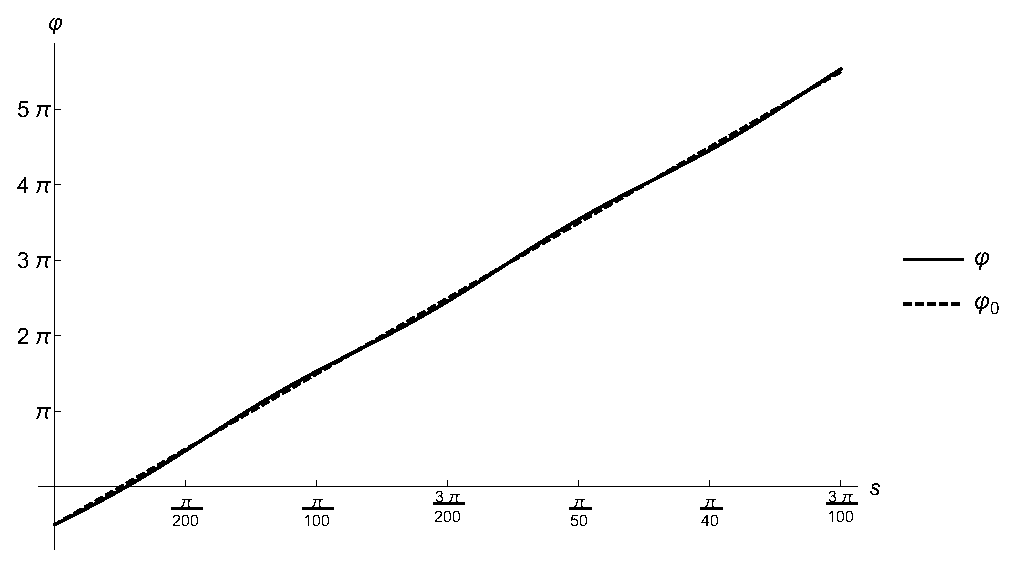
\includegraphics[scale=0.52]{RAppW98R1L2.eps}
\subcaption{Rozwiązanie przybliżone dla $\omega=0,98$}\label{fig:3a1}
\end{minipage}%
\begin{minipage}[b]{.5\linewidth}
\centering
\includegraphics[scale=0.52]{RNumW98R1L2.eps}
\subcaption{Rozwiązanie pełne dla $\omega=0,98$}\label{fig:3n1}
\end{minipage}
\begin{minipage}[b]{.5\linewidth}
\centering
\includegraphics[scale=0.52]{RAppW99R1L2.eps}
\subcaption{Rozwiązanie przybliżone dla $\omega=0,99$}\label{fig:3a2}
\end{minipage}%
\begin{minipage}[b]{.5\linewidth}
\centering
\includegraphics[scale=0.52]{RNumW99R1L2.eps}
\subcaption{Rozwiązanie pełne dla $\omega=0,99$}\label{fig:3n2}
\end{minipage}
%\begin{minipage}[b]{.5\linewidth}
%\centering
%\includegraphics[scale=0.52]{RAppW993R1L2.eps}
%\subcaption{Rozwiązanie przybliżone dla $\omega=0,993$}\label{fig:3a3}
%\end{minipage}%
%\begin{minipage}[b]{.5\linewidth}
%\centering
%\includegraphics[scale=0.52]{RNumW993R1L2.eps}
%\subcaption{Rozwiązanie pełne dla $\omega=0,993$}\label{fig:3n3}
%\end{minipage}
\caption{Porównanie rozwiązania przybliżonego z rozwiązaniem pełnym
dla fazy zegara $\varphi$ w ruchu po okręgu przy
$\ell=0,01$ i $R=1$ dla różnych prędkości $\omega$. 
Linią przerywaną zaznaczono fazę 
$\varphi_0$ w układzie bez przyspieszeń.}\label{fig:3}
\end{figure}
\newpage
\subsection{Analiza modelu pod kątem pomiaru.}
Najprostszym obiektem, dla którego można użyć modelu zegara 
idealnego wydaje się być elektron. 
Oszacujemy rząd wielkości przyspieszenia, dla którego spodziewamy się 
obserwowalnych odstępstw od hipotezy zegara.
Za~$\ell$~możemy podstawić wielkość o wymiarze metra 
charakterystyczną dla elektronu - długość 
Komptonowską fali~\eqref{compton_electron}. 
Wtedy przyspieszenie charakterystyczne dla elektronu 
wynosi~\eqref{ac_electron}.
Dla porównania energie elektronów otrzymywane 
w akceleratorach liniowych są rzędu 
kilku-kilkunastu $\si{\giga\electronvolt}$.
Dla szacowania przyjmiemy gradient przyspieszenia rzędu
kilku $ \si{\giga\electronvolt \per \metre}$~\cite{Ghotra2015}.
Rząd wielkości przyspieszenia 
szacujemy jako~\eqref{acceleration_electron_nowadays}.
\begin{align}\label{compton_electron}
\lambda_e  \approx 2,426 \cdot 10^{-10} \si{\centi\metre} ,
\end{align}
\begin{align}\label{ac_electron}
\alpha_c \approx 8,244\cdot 10^{9} \si{ \centi\metre^{-1}} ,
\end{align}
\begin{align}~\label{acceleration_electron_nowadays}
\alpha \approx 10^2 \si{\centi\metre^{-1}} .
\end{align}

Komptonowska długość fali protonu wynosi~\eqref{compton_proton}. 
Przyspieszenie charakterystyczne dla protonu równe~\eqref{ac_proton}.
%$\alpha_c \approx 1,36\cdot 10^{34} 
%\si{\centi\meter^2 \per \second}$.
Energie protonów osiągane w CERN są rzędu 
$7 \si{\tera\electronvolt}$~\cite{CERN}. Wtedy 
proton doświadczy przyspieszenia
rzędu~\eqref{proton_acceleration}.
Porównując rzędy wielkości przyspieszeń stwierdzamy, 
że osiągalne w tej chwili przyspieszenia nie są wystarczające 
do sprawdzenia hipotezy.
\begin{align}\label{compton_proton}
\lambda_p  \approx 1,321 \cdot 10^{-13} \si{\centi\metre} ,
\end{align}
\begin{align}\label{ac_proton}
\alpha_c \approx 7,57 \cdot 10^{12} \si{ \centi\metre^{-1}} ,
\end{align}
\begin{align}~\label{proton_acceleration}
\alpha \approx 124  \si{\centi\metre^{-1}} .
\end{align}
